\documentclass[11pt]{article}
\usepackage{times}
\pagestyle{empty}
\parindent 0px
\usepackage{geometry}
 \geometry{
 a4paper,
 total={170mm,257mm},
 left=20mm,
 top=20mm,
 }
 
\title{CS5691: Assignment 2}
\author{Akshat Meena (CS19B052) \\ Rohit Bhagat (CS19B038)}
\date{}
\usepackage{graphicx}
\graphicspath{ {../Plots/} }

\begin{document}
\maketitle

\begin{center}
\begin{Large}
A. Regression
\end{Large}
\end{center}

\begin{enumerate}
	\begin{large}
	\item \textbf{1D Dataset}
	\end{large}
	
	\begin{itemize}
		\item \textbf{Least square regression}\\	
		We experiment with different sample size keeping the complexity constant. We plot the least square regression for N = 20, 50, 100, 200 and M = 7. We observe that for lower value of N, the curve isn't smooth and may over-fit too depending on M. As we start increasing N, the curve starts getting smoother.
	\begin{figure}[h]
	\caption{
	\begin{small}
	Plots for N = 20, 50, 100, 200 and M = 7.
	\end{small}
	}
	\centering
	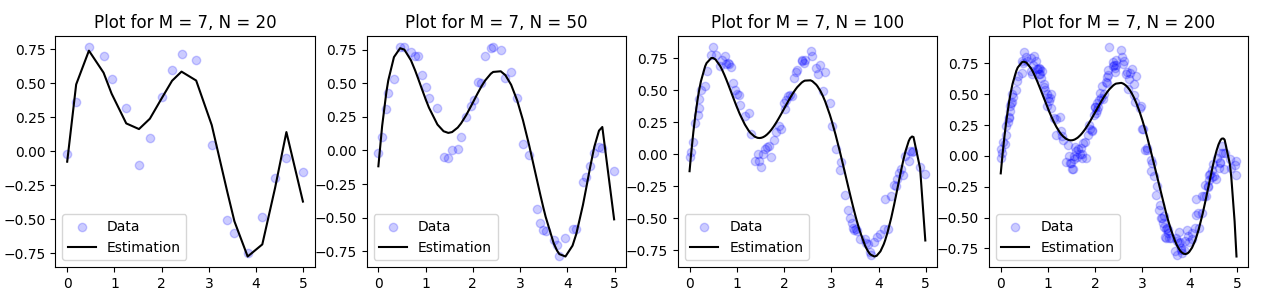
\includegraphics[scale=0.55]{1A}
	\end{figure}\\
	Then we experiment with different model complexity keeping the size same.We plot the least square regression for M = 1, 5, 10 ,22 and N = 1000. We observe the for low model complexity the curve is not able to fit properly but as the M increase it starts fitting the data, if we increase the model complexity more then the curve start over-fitting.
	\begin{figure}[h]
	\caption{
	\begin{small}
	Plots for M = 1, 5, 10, 22 and N = 200.
	\end{small}
	}
	\centering
	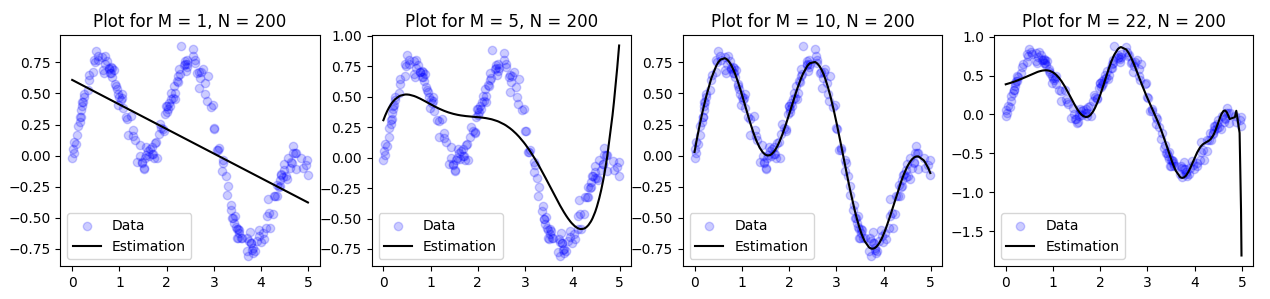
\includegraphics[scale=0.55]{1B}
	\end{figure}\\
	
	\item \textbf{Ridge regression}\\
		We experiment with different regularization parameter($\lambda$) keeping the M and N constant. We plot the Ridge regression for ln($\lambda$) = -100, -10, -1, 0. The regularization parameter helps dealing with over-fitting.
	\begin{figure}[h]
	\caption{
	\begin{small}
	Plots for ln($\lambda$) = -100, -10, -1, 0 and M = 10 and N = 200.
	\end{small}
	}
	\centering
	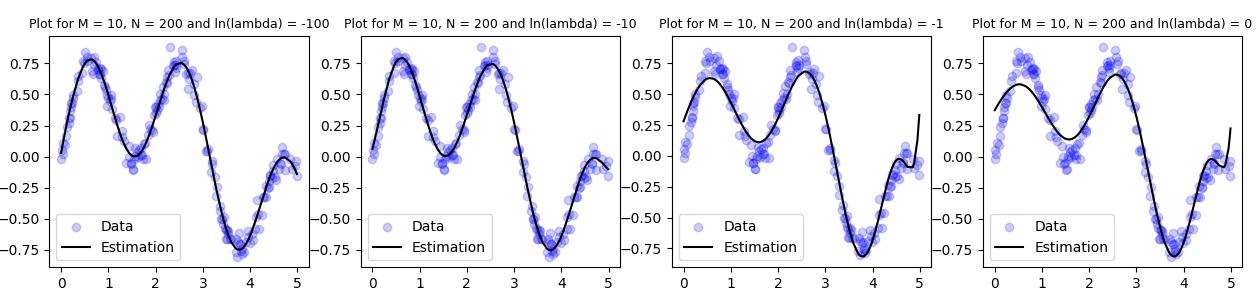
\includegraphics[scale=0.55]{1C}
	\end{figure}
	\item \textbf{Error plots}\\
	We also plot the error of our model for training and development sets vs model complexity and the regularization
parameter. In the plot with varying M we see that initially the error decreases but later due to over-fitting it starts increasing. Similarly in the plot with varying regularization parameter
however the plot shifts from over-fit to under-fit.
	\begin{figure}[h]
	\caption{
	\begin{small}
	Error plots
	\end{small}
	}
	\centering
	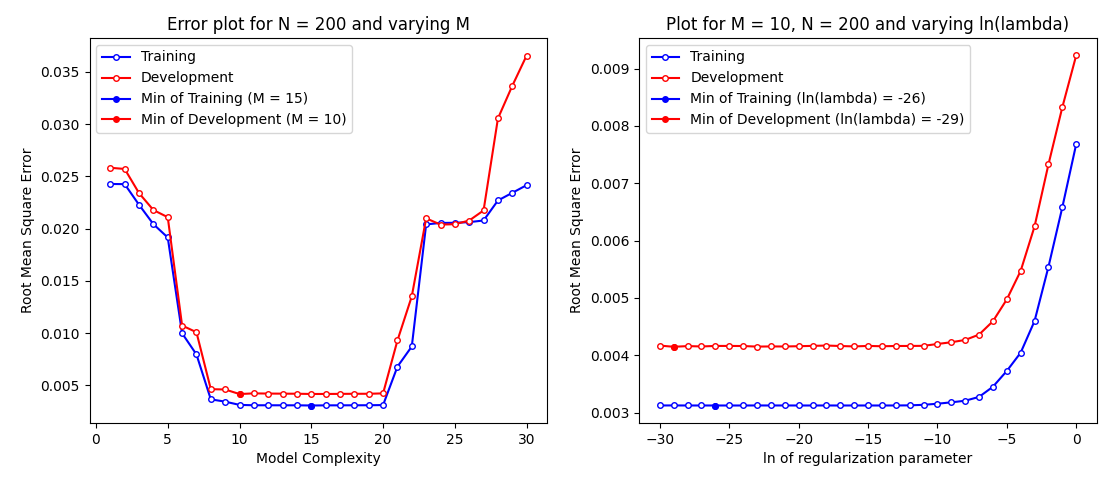
\includegraphics[scale=0.45]{1D}
	\end{figure}\\
	We can see that we can get best trained model for Model complexity(M) = 10 and regularization parameter($\lambda$) = $e^{-29}$
	\end{itemize}
	
	\begin{large}
	\item \textbf{2D Dataset}
	\end{large}
	
	\begin{itemize}
		\item \textbf{Least square regression}\\	
		We experiment with different sample size keeping the complexity constant. We plot the least square regression for N = 20, 100, 500, 1000 and M = 7. We observe that for lower value of N, the curve isn't smooth and may over-fit too depending on M. As we start increasing N, the curve starts getting smoother.
	\begin{figure}[h]
	\caption{
	\begin{small}
	Plots for N = 20, 100, 500, 1000 and M = 7.
	\end{small}
	}
	\centering
	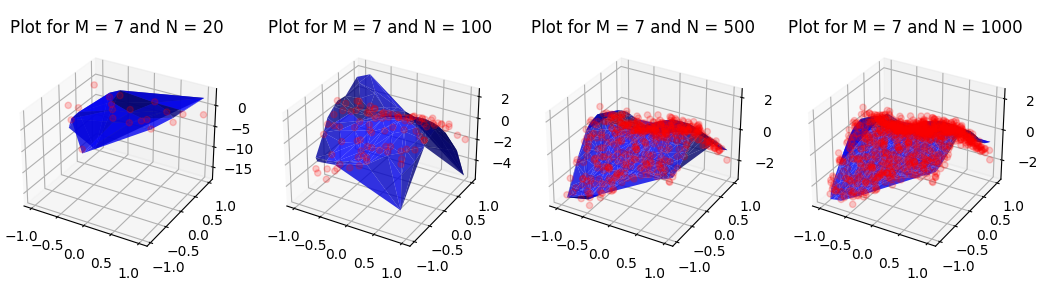
\includegraphics[scale=0.55]{2A}
	\end{figure}\\
	Then we experiment with different model complexity keeping the size same.We plot the least square regression for M = 1, 5, 10 ,20 and N = 1000. We observe the for low model complexity the curve is not able to fit properly but as the M increase it starts fitting the data, if we increase the model complexity more then the curve start over-fitting.
	\begin{figure}[h]
	\caption{
	\begin{small}
	Plots for M = 1, 5, 10, 20 and N = 200.
	\end{small}
	}
	\centering
	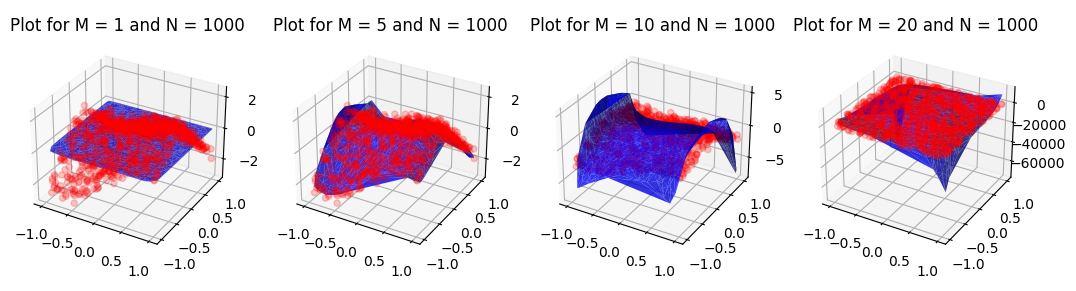
\includegraphics[scale=0.55]{2B}
	\end{figure}\\
	\item \textbf{Ridge regression}\\
		We experiment with different regularization parameter($\lambda$) keeping the M and N constant. We plot the Ridge regression for ln($\lambda$) = -100, -10, -1, 0. The regularization parameter helps dealing with over-fitting.
	\begin{figure}[h]
	\caption{
	\begin{small}
	Plots for ln($\lambda$) = -100, -10, -1, 0 and M = 7 and N = 1000.
	\end{small}
	}
	\centering
	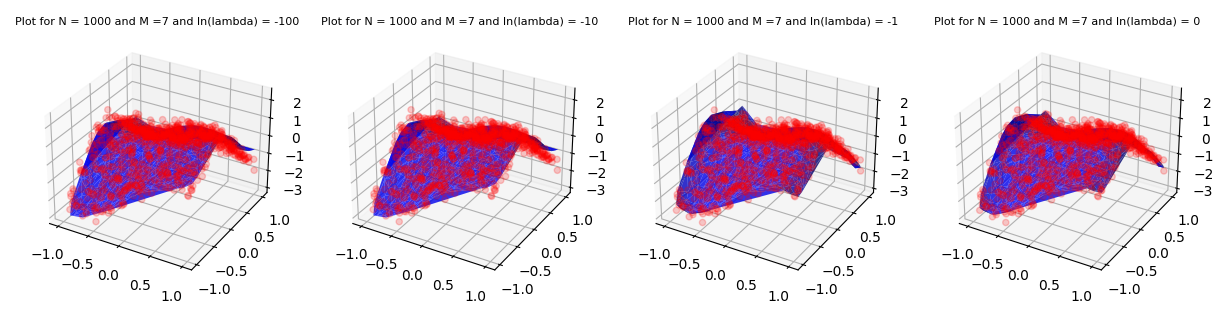
\includegraphics[scale=0.55]{2C}
	\end{figure}
	\item \textbf{Error plots}\\
	We also plot the error of our model for training and development sets vs model complexity and the regularization
parameter. In the plot with varying M we see that initially the error decreases but later due to over-fitting it starts increasing. Similarly in the plot with varying regularization parameter
however the plot shifts from over-fit to under-fit.
	\begin{figure}[h]
	\caption{
	\begin{small}
	Error plots
	\end{small}
	}
	\centering
	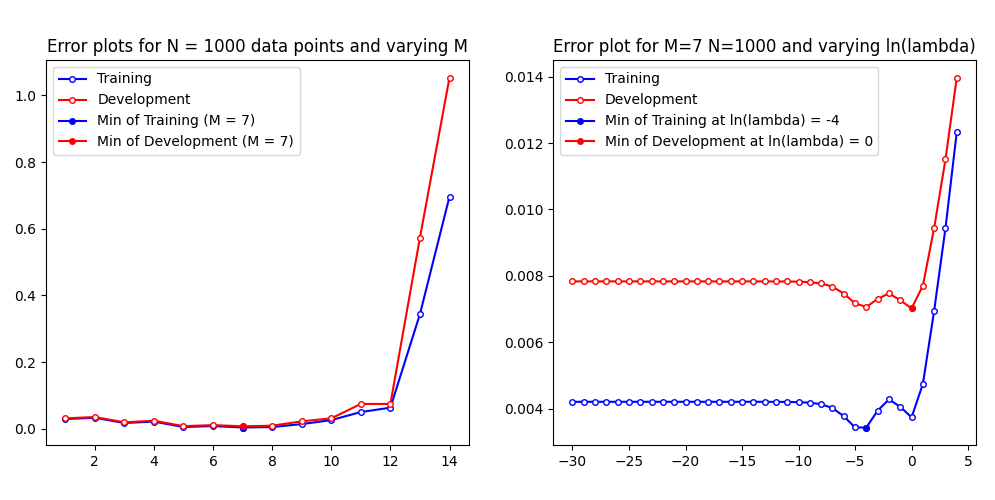
\includegraphics[scale=0.45]{2D}
	\end{figure}\\
	We can see that we can get best trained model for Model complexity(M) = 7 and regularization parameter($\lambda$) = $e^{0}$
	\end{itemize}
	
\end{enumerate}

\end{document}